\section {Linear algebra}

The linear algebra is the algebra of matrices. Matrices form a vector-space, an inner-product-space and an algebra. 


\subsection{Linear Transformations}

By accident, I created a transformation that results in a so called \hyperlink{https://en.wikipedia.org/wiki/Lissajous_curve}{Lissajous curve}.

\begin{figure}
  \caption{line to tr}
  \centering
    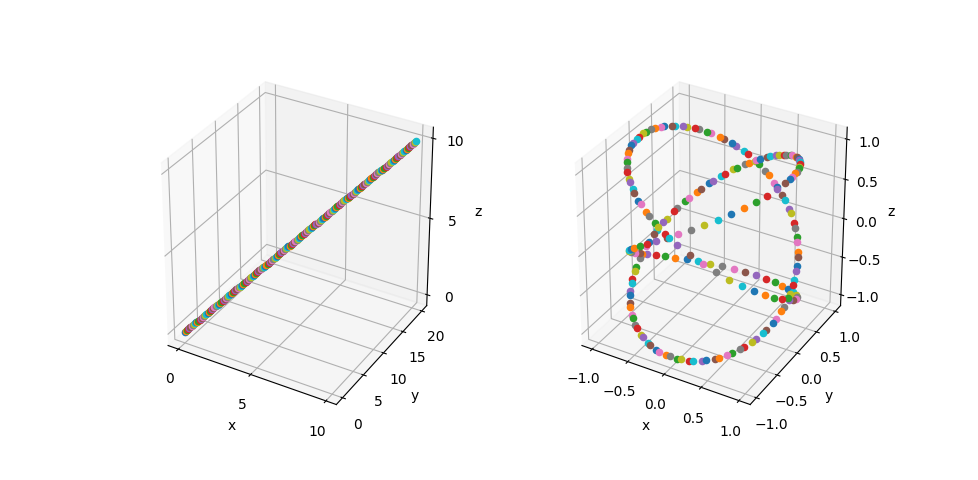
\includegraphics[width=0.8\textwidth]{images/transform.png}
\end{figure}



\begin{lstlisting}[language=python]
import numpy as np
from collections import namedtuple as nt
from infix import or_infix
from math import sin, cos, atan, tan, exp, log

Point = nt("Point", "x,y,z")

@or_infix
def vplus(point1, point2):
    x = point1.x + point2.x
    y = point1.y + point2.y
    z = point1.z + point2.z
    return Point(x, y, z)

@or_infix
def sprod(s, point):
    x = s * point.x
    y = s * point.y
    z = s * point.z
    return Point(x, y, z)

def Line(t):
    return Point(0, 0, 0) |vplus| ( t |sprod| Point(1, 2, 1) )

def transform(point):
    x = cos(point.x + point.y)
    y = sin(point.y + point.z)
    z = cos(point.z + point.x)
    return Point(x, y, z)

line = [Line(t) for t in np.arange(0.0, 10.0, 0.05)]
line2 = [transform(p) for p in line]
\end{lstlisting}



% Hier kommt ein Haufen Zeug aus Kap 8-9 von Macdonnald

\paragraph{A linear transformation is a change of base when} ....




























\subsection{Solveable systems}
If there are more variables than equations, the system is underdetermined. If there are more eqations than variables, the system is overdetermined. A potentially solveable system is one where there are equally many variables as equations. But even then we must distinguish two cases. 

\subsubsection{Solving well determined systems}
There are two cases: a system is either consistent or inconsistent. The follwing statements are all equivalent, meaning that any one of them is related to any other one in an if-and-only-if way. 

\begin{itemize}
    \item the system is consistent
    \item the matrix is invertible
    \item the determinant is nonzero
    \item there is exactly one sollution
\end{itemize}

We proof a few of those equivalences just for the hell of it. 

\begin{proof} There is exactly one solution if and only if the determinant is nonzero. \\
    \subprf{}{$|A| = 0 \iff \thereis ! \vec{x} : A \vec{x} = \vec{b} $}{
    
    }
\end{proof}

On the other hand, in the inconsistent case, the follwing statements are equivalent:

\begin{itemize}
    \item the system is inconsistent
    \item the matrix is singular (aka. noninvertible)
    \item the determinant equals zero
    \item one (or more) row (or column) is lineraly dependent of the others
\end{itemize}

\subsubsection{Solving overdetermined systems: least squares}


\subsubsection{Solving underdetermined systems: geometric bodies}
I like to think of underdetermined systems as (linear) geometric bodies, written in their parameterized form. A line in $\reals^3$ is described by a $3 \times 1$ matrix (or rather, it's column space), a plane in $\reals^3$ by a $3 \times 2$ matrix. However, it is important to note one distinction: geometric objects don't need to go through the origin, a matrix system however does. A line that does not go through the origin needs a base vector, like so: 

$$\vec{x} = \begin{bmatrix} \vec{d} \end{bmatrix} \begin{bmatrix} \alpha \end{bmatrix} + \vec{b}$$ 

A plane that does not go through the origin also needs a base vector $\vec{b}$, like so: 

$$\vec{x} = \begin{bmatrix} \vec{p}_1 && \vec{p}_2 \end{bmatrix} \begin{bmatrix} \alpha  \\ \beta \end{bmatrix} + \vec{b}  $$



Here is a problem that bothered me for a while: a line needs one parameter, a plane two. An ellipsoid, too, needs two parameters. Are there any linear geometric objects in $\reals^3$ that require more than three parameters? The answer is: no. Here is the proof. 

\begin{proof}
    For any $3 \times 4$ matrix, there is a $3 \times 3$ matrix that has the same column space, that is, that describes the same geometrical body. \\
    
    \subprf{}{$\forall A(3 \times 4) \thereis A'(3 \times 3): \collspace{A} = \collspace{A'}$}{

        \subprf{Let $A_0(3 \times4)$.}{$\thereis A': \collspace{A_0} = \collspace{A'}$}{
        
            We know from \ref{proofBaseSizeEqualsSpaceDimension} that $\thereis \vec{a}_0 \in A_0: \vec{a}_0:ld$. So Try $A' = A_0/\vec{a_0}$.
            
            Indeed, now $A_0$ and $A'$ both form a base of the same space. So they must have the same column space. 
        }    

    }
\end{proof}

However, there are \emph{non}linear objects in $\reals^3$ that require more than three parameters! Many curves in 3d require many parameters. \emph{But} those curves don't form a vector-space, while lines and planes do (as long as they go through the origin). 


\subsubsection{Useful properties of the determinant}

\paragraph{The size of the determinant} can be seen as the scaling-factor of the transformation described by the matrix $A$.

\paragraph{The size of the determinant} is a measure of how much linearly independent the rows/cols of $A$ are. The size of the determinant equals the size of the (hyper-)parallelogram spanned by the columns. If two vectors are almost linearly dependent, they will be almost parallel, leading to a very small area of the parallelogram. So if you have a small determinant, your columns are almost dependent. If you have a large one, your colums are very orthogonal. 

\subsubsection{Summary}
\begin{table}[ht]
\centering
\caption{Influence of rank on solutions}
\begin{tabular}{@{}llll@{}}
\toprule
                                                                                      & m \textless n                             & m = n & m \textgreater n                                 \\ \midrule
\rowcolor[HTML]{96FFFB} 
\cellcolor[HTML]{96FFFB}                                                              & n - m free variables                      &       &                                                  \\
\rowcolor[HTML]{96FFFB} 
\multirow{-2}{*}{\cellcolor[HTML]{96FFFB}r \textless m}                               & m – r conditions on $b \in \collspace{A}$ &       &                                                  \\
                                                                                      & 1 pivot per row                           &       &                                                  \\
                                                                                      & n – r = n – m free variables              &       &                                                  \\
\multirow{-3}{*}{\begin{tabular}[c]{@{}l@{}}r = m \\ (full row rank)\end{tabular}}    & 0 conditions on $b \in \collspace{A}$     &       & X                                                 \\
\rowcolor[HTML]{96FFFB} 
\cellcolor[HTML]{96FFFB}                                                              &                                           &       & m – r conditions on $b \in \collspace{A}$        \\
\rowcolor[HTML]{96FFFB} 
\multirow{-2}{*}{\cellcolor[HTML]{96FFFB}r \textless n}                               &                                           &       & n – r free variables                             \\
                                                                                      & X                                         &       & 1 pivot per column                               \\
                                                                                      &                                           &       & m – r = m – n conditions on $b \in \collspace{A}$ \\
\multirow{-3}{*}{\begin{tabular}[c]{@{}l@{}}r = n \\ (full column rank)\end{tabular}} &                                           &       & 0 free variables, thus $\nullspace{A} = \{0\}$     \\ \cmidrule(l){1-4} 
\end{tabular}
\end{table}















\subsection{Allowed operations and solving Ax = b}

\subsubsection {Solution space} 


\subsubsection  {rops and cops as matrix multiplication}
$$ \rops(A) = \rops(I) A = R A$$
$$ \cops(A) = A \cops(I) = A C$$

\subsubsection{rops don't change \nullspace{A}}

\begin{theorem}
  Row-operations on $A$ don't change \nullspace{A}. 
\end{theorem}

\begin{proof}
    \subprf {Let $A' = \rops(A) = RA$} {\nullspace{A} = \nullspace{A'}} {
        \subprf {Let $x_0: Ax_0 = 0$} {$\exists y_0: A'y_0 = 0$} {
            \subprf {Try $y_0 = x_0$} {$A'y_0 = 0$} {
                $RAy_0 = 0$
            }
        } \\
        \subprf {Let $y_0: A'y_0 = 0$} {$\exists x_0: Ax_0 = 0$} {
            \subprf {} {$\exists x_0: R^{-1} A' x_0 = 0$} {
                \subprf {Try $x_0 = y_0$} {$R^{-1} A' x_0 = 0$} {
                    $R^{-1} A' x_0 = 0$
                }
            }
        }
    } 
\end{proof}

Therefore, when searching for the special solutions to a problem $Ab = 0$, we can use Gauss-Elemination and RREF without any problems.

\subsubsection {cops don't change C(A)}

\subsubsection {rops don't change C(A) if A is invertible }

\subsubsection {Ax = b reduces to A'x' = 0}

\begin{theorem}
  A problem of the form $Ax = b$ can be re-expressed as $A'x' = 0$, where $A' = [A, -b]$ 
\end{theorem}

\begin{proof}
    \subprf {} {$A x = b$ can be re-expressed as $A'x' = 0$} {
        $ A x = b $ \\
        $ A x -b = 0 $ \\
        $ A_1 x_1 + A_2 x_2 + ... -b = 0 $ \\
        Let $A' = [A, b]$ and $x_{n+1} = -1$. Then: \\
        $ A' x' = 0 $ \\
        Now we can use the nullspace of $A'$ to find the solutionspace of $A$. \\
        $ \nullspace{[A b]} = \{x' | [A b]x' = 0\} $ \\
        $ = \{x' | A x'_{1:m} = -b x'_{m+1}\} $ \\
        A subset of that nullspace equals the solutionset for $A x = b$: \\
        $ \nullspace{[A b]}_{[x'_{m+1} = -1]} = \{x'| A x'_{1:m} = b \} $ 
    }   
\end{proof}


\subsubsection{Solving Ax = b}

\begin{theorem}
  If we can only find any one particular solution $x_p$ such that $A x_p = b$, then we get the whole solutionspace as $\nullspace{A} + x_p$.
\end{theorem}

\begin{proof}
    \subprf{Let $x_p: A x_p = b$.}{$\solspace{A x = b} = \nullspace{A} + x_p$}{
        We'll make use of the fact that $\nullspace{A} + x_p = \{ x + x_p | A x = 0 \} = \{ x | A x = A x_p \}$ \\
        \subprf{Let $x_0 \in \nullspace{A} + x_p $.}{$x_0 \in \solspace{A x = b}$, i.o.w. $A x_0 = b$}{
            $ x_0 \in \nullspace{A} + x_p $ \\
            $ x_0 \in \{ x + x_p | A x = 0 \} $ \\
            $ x_0 \in \{ x | A (x - x_p) = 0 \} $ \\
            Thus $ A x_0 = A x_p $ \\
            Since $A x_p = b$, it must be that $ A x_0 = b $.
        }
        \subprf{Let $x_0 \in \solspace{A x = b}$.}{$x_0 \in \nullspace{A} + x_p$, i.o.w. $A x_0 = A x_p$}{
            Because $x_0 \in \solspace{A x = b}$, we have $A x_0 = b$. \\
            Also, it was given that $A x_p = b$.
        }
    }
\end{proof}















\subsection{The four fundamental subspaces of linear algebra}

We can now print an overview of the different spaces that are associated with a matrix $A$ of dimension $m \cdot n$ and rank $r$.

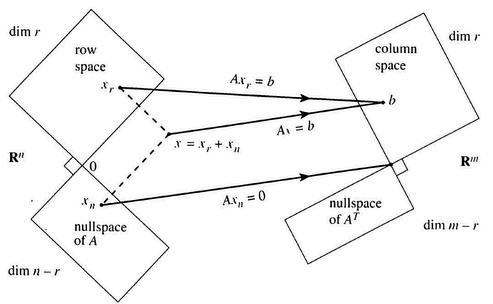
\includegraphics[width=0.8\linewidth]{images/four_spaces.png}

The rowspace of $A$ can be visualized using the line-intersection view of matrix-equations: it contains all the points that lie in the intersection of all the lines that make up the matrix. The columspace of A can be visulaized using the vector-image of A: it contains all the points that are spanned by A. 
Notice how we included the previous theorem: any combination $x$ of a particular sollution $x_r$ and any vector in the nullspace $x_n$ is also a solution.


\subsection{Spaces and eigenthingies}

\begin{definition}
Let $W$ be a space. Then $V \subseteq W$ is a subspace, if: 
    \begin{itemize}
        \item $\forall v_1, v_2 \in V: v_1 + v_2 \in W$
        \item $\forall v \in V: \forall r \in R: rv \in V$
    \end{itemize}
\end{definition}


\begin{definition}
    $B$ is linearly independent if $\forall b \in B: b \neq \sum r_n b_n$, with $b_n \in B/b$. 
\end{definition}

\begin{theorem}
  A better definition could be stated as such: $B$ is linearly independent, if the only solution to $Bx = 0$ is the zero-vector.
\end{theorem}

\begin{proof}
    \subprf{}{$( Bx = 0 \leftrightarrow \forall x_n = 0 ) \leftrightarrow (\forall b \in B: b \neq \sum r_n b_n, b_n \in B/b)$}{
        todo.
    }
\end{proof}

\begin{definition}
    Let $V$ be a subspace. $B \subseteq V$ is a basis for $V$ if $B$ is linearly independent and $\forall v \in V: v = \sum r_n b_n$, with $b_n \in B$
\end{definition}


TODO: definition and deduction eigenvalues

\subsubsection{Orthogonal matrices}
TODO: definition orthogonal

\begin{theorem}
    If $A$ is orthogonal, than $A^{-1} = A^T$.
\end{theorem}


\subsubsection{Matrix factorisation}

\paragraph{Eigenvalue decomposition}

$$ A = V \Lambda V^{-1} $$

\paragraph{Singular value decomposition} is eigenvalue decomposition, generalized to non-square matrices.

$$ A = U \Sigma V^T $$

SVD is related to EVD like this: 

\begin{equation}
    A^T A &= V \Sigma^T U^T U \Sigma V^T \\
          &= V \Sigma^T \Sigma V^T
\end{equation}

This makes the entries of $\Sigma$ the squares of the eigenvalues of the matrix $A$.

\paragraph{Nonnegative matrix factorisation}: Consider a dataset $A$, mapping people (rows) to properties (columns). You are looking for some hidden, small set of features, that groups of people have in common. 
In neural networks we can reconstruct images from a minimal amount of hidden features by funnelling the image through a very small hidden layer out to a large output layer. We can do the very same thing here!
$$ A = U V $$
Where $A$ has dimension $r \cross c$, $U$ associates people with their hidden features/groups $r \cross f$ and $V$ associates features/groups with the properties $f \cross c$.